\hypersetup{pageanchor=false}
\begin{titlepage}
\centering
\vspace*{5mm}
{\Large B.Tech Project Report\par}
\vspace{8mm}
{\fontsize{29}{34}\selectfont\bfseries Aegis Perception\par}
\vspace{5mm}
{\Large Multi-Weather Restoration\par and Edge Perception\par}
\vspace{8mm}
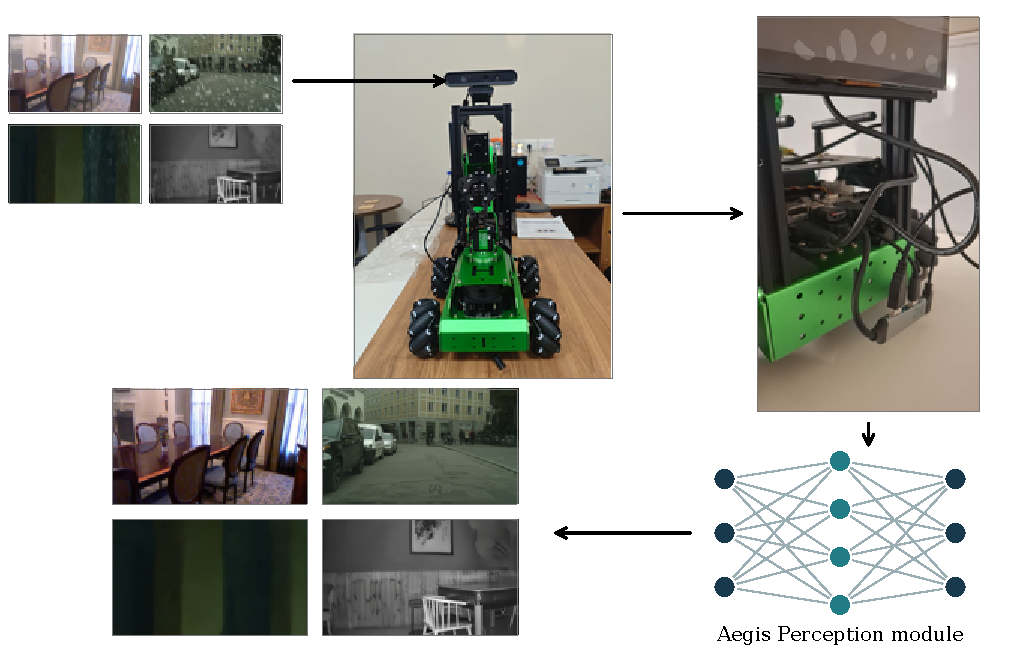
\includegraphics[width=\textwidth]{figures/cover_pipeline.pdf}
\vspace{5mm}
{\large
\begin{tabular}{@{}lr@{}}
Chitraksh & CS23B054\\[3mm]
Sudhanva & CS23B051\\[3mm]
Rishikesh & CS23B015
\end{tabular}\par}
\vspace{8mm}
{\large\textbf{Guide: Dr Vishnu Chalavadi}\par}
\vfill
{\large Indian Institute of Technology Tirupati\par}
\vspace{5mm}
{November 2026\par}
\vspace{3mm}
\end{titlepage}
\hypersetup{pageanchor=true}
\pagenumbering{roman}
\section*{Abstract}\addcontentsline{toc}{section}{Abstract}
Adverse-weather restoration must be judged by what it preserves for a vision
system as well as by its similarity to a clean image. This project studies
rain, fog, snow and smoke through three linked evaluations: a controlled
paired-image benchmark, fixed-detector comparisons, and execution on the
original 4\,GB Jetson Nano.

Six restoration systems are trained under a shared split and evaluation
protocol, with 18,610 training, 2,011 validation and 2,334 test pairs. Their
initialization sources differ. Restormer leads the balanced native-resolution
comparison at 32.58\,dB PSNR and 0.93 SSIM. Eight continuation arms test
spatial and detail adapters and auxiliary losses against matched further
training. No arm satisfies the validation replacement rule, so the original
epoch-51 checkpoint remains selected.

Downstream results depend on the complete processing path. In the earlier
72-image local DAWN pilot, pooled AP$_{50:95}$ rises from 29.97\% to 32.86\%,
with gains concentrated in fog. In the separately measured Nano cascade,
pooled AP falls from 29.59\% to 14.50\%. Labelled replay reaches only
0.61--0.62 frames/s with restoration, compared with 6.55--7.28 frames/s for
YOLO alone, while input energy increases to 11.35--11.59\,J/frame. Matched local
resolution controls demonstrate that both resampling and restoration can
change detections. An offline 8-bit weight grid fails two numerical-agreement
fixtures and retains FP32 storage and execution.

Six experimental phases are complete. The current exploratory phase investigates
RAMiT + YOLOv12 edge deployment, informed by the measured Restormer/YOLOv8n
limitations. The work establishes a reproducible comparison and identifies practical
failure modes. It does not establish universal detector improvement,
real-time edge operation, or an accepted INT8 acceleration. Single training
seeds, limited smoke backgrounds and short device trials bound the conclusions.

\textit{Keywords:} image restoration, adverse weather, Restormer, object
detection, controlled evaluation, Jetson Nano, quantization.
\begingroup
\setlength{\parskip}{0pt}
\tableofcontents
\endgroup
\clearpage
